\documentclass[12pt]{TDP005mall}
\usepackage{graphicx}
\usepackage{unicode-math}


\newcommand{\version}{Version 1.0}
\author{Elliot Johansson, \url{elljo130@student.liu.se}\\
  Lukas Freyland, \url{lukfr510@student.liu.se}\\
  Nadim Lakrouz, \url{nadla777@student.liu.se}}
\title{Designspecifikation}
\date{2022-11-25}
\rhead{Elliot Johansson\\
Lukas Freyland\\
Nadim Lakrouz}



\begin{document}
\projectpage
\section{Revisionshistorik}
\begin{table}[!h]
\begin{tabularx}{\linewidth}{|l|X|l|}
\hline
Ver. & Revisionsbeskrivning & Datum \\\hline

1.0 & Första utkast & 2022-11-25 \\\hline
\end{tabularx}
\end{table}

\section{Player}
Syftet med playerklassen är att representera den karaktär spelaren styr. Spelaren kan gå runt med karaktären och samtidigt använda magiska formler i form av cirklar runt spelaren. Formlerna kommer att följa spelarens rörelser. Spelaren kan röra sig runt hela spelplanen men inte utanför. 

Funktionen regenerate\_mana kommer sakta återställa manapoäng med sf:Clock och sf::Time. 
Hitpoint och mana visar spelaren hur mycket liv hen har kvar samt om hen kan använda en magisk formel.
Hitpoint och mana visas i form av ''bars'' som ändras i storlek procentuellt med hur många hitpoints samt mana finns kvar.


\subsection{}

\begin{itemize}
    \item double hitpoint\{\} - Håller antalet ''hitpoints'' spelaren har vilket är spelarens liv.
    \item int hitpointMax\{\} - Håller ett fast värde på det maximala antal ''hitpoints''. Används för att få fram ett procentuellt värde av hur många hitpoints som finns.
    
    \item double HpPercent\{\} - Ett procent värde som används för att veta hur stor HP-baren ska vara relaterbart med hur många ''hitpoints'' spelaren har kvar.
    
    \item double mana\{\} - Håller antalet mana spelaren har. Mana bestämmer om spelaren kan använda en trollformell.
    
    \item double manaMax\{\} - Ett fast värde på det maximala antalet mana spelaren har. Används för att få fram ett procentuellt värde av hur mycket mana som finns.
    
    \item double ManaPercent\{\} - Antal procent av mana jämfört med manaMax. Används för att veta hur stor Mana-baren ska vara relaterbart till antalet mana.
    
    \item sf:Clock m\_clock - sfml variabel för att hantera tiden.
    
    \item sf::Time m\_elapsed - sfml variabel för att hantera tiden.
    
    \item void RestartClock() - Startar om tiden. Mana ska uppdateras en gång varje intervall och RestartClock() startar om intervallet.
    
    \item void updatePlayerGUI() - Updaterad ''Graphical User Interface'' för spelarens Hp- och Mana-bar.
    
    \item int set\_hp() - Ändrar privata variabeln ''hitpoint'' när spelaren ska förlora eller få tillbaka hitpoints.
    
    \item int get\_hp() - Hämtar privata variabeln hitpoint för att bl.a. stoppa spelaren från att få mer hitpoints än hitpointMax.
    
    \item int get\_mana() - Hämtar privata variabeln mana för att bl.a. se till att trollformler bara kan användas när spelaren har mana.
    
    \item void regenerate\_mana() - Använder sig av m\_clock och m\_elapsed för att öka privata variabeln mana ett bestämt antal varje intervall.
    
    \item void update() - uppdaterar mana, position, återställer klockan och anroppar updatePlayerGUI().
    
    \item void renderPlayerGUI(sf::RenderTarget \& target) - Renderar spelarens Hp- och Mana-bars med bestämd längd och position.
    
    \item void render(sf::RenderTarget \& target) - Renderar spelarens karaktär.
    
    \item void resetPlayer() - Återställer spelaren om spelaren skulle dö.

    
    
\end{itemize}
\clearpage


\section{Enemies}
''Enemies'' klassens syfte är att representera fienderna som i intervaller kommer förflytta sig mot spelaren på spelplanen. Vid kollision med magiska formler så kommer det påverka fienderna på olika sätt. Exempelvis kommer de antingen dö eller bli stoppade beroende på vilken magisk formel som spelaren använder.

Vid kollision med spelaren tar spelaren skada fram tills spelaren inte längre är i kontakt med fienden. 
\subsection{}

\begin{itemize}
    \item float size - Storlek på fiender. Bestämmer radien på circle.
    
    \item double xMovement - Fienders rörelse i X-led.
    
    \item double yMovement - Fienders rörelse i Y-led.
    
    \item sf::CircleShape circle{size} - Formen på en fiende. Används som hitbox för att rita ut fienden.
    
    \item sf::Vector2f location{} - Förvarar fienders position.
    
    \item sf::Texture texture - Innehåller Fienders textur.
    
    \item std::vector\quad $<$sf::Texture*$>$ textures - En container som förvarar alla fienders olika texturer.

    \item Enemy(float size, sf::Texture \&texture) - Skapar ett fiende objekt med bestämd storlek och textur och sätter texturen till circle.
    
    \item void update(sf::Vector2i pos) - Uppdaterar fienders position enligt xMovment och yMovment. 
    
    \item void render(sf::RenderTarget \& target) - Renderar circle.
    
    \item sf::CircleShape getCircle() - Hämtar circle.
    
    \item void setLocation(float x, float y) - Bestämmer positionen av fienderna.
    
    \item sf::Vector2f getLocation() - Hämtar position av fiender
    
    \item int getDistanceCircles(Enemy\& otherEnemy) - Hämtar avståndet mellan två fiender.
    
    \item bool checkCollision(Enemy\& otherEnemy) - Kontrollerar om två fiender överlappar varandra med hjälp av getDistanceCircles(Enemy\& otherEnemy) funktionen.
    
    \item double getxMovement() - Hämtar rörelser i X-led.
    
    \item double getyMovement() - Hämtar rörelser i Y-led.
    
    \item void setMovement(sf::Vector2i pos) - Bestämmer vilket riktning fiender ska gå mot då de ska alltid röra sig mot spelaren.
    
    \item sf::Vector2f spawnPoint() - Bestämmer var fienders skapas på spelplanen.
\end{itemize}


\section{Diskussion och filhantering}
Vår design är uppbyggd av en Engine som har kontroll över flera ''states''. De här ''statsen'' är Menu\_state, Game\_state och Gameover\_state, alla ärver av Base\_state. De olika ''statsen'' gör det lätt att hantera olika spelfaser genom att skapa olika dedicerade objekt i de olika ''statsen''. Det gåt att dela upp hanteringen av objekten så att allt inte ligger på ett och samma ställe. Till exempel det är onödigt att ha en Player-objekt i Menu\_state då Player-objekten ändast behöver vara i Game\_state.

Vårt program använder sig av en ''resource\_manager'' som kan hantera olika typer av filer. På så sätt behöver vi bara använde en funktion för att hantera alla externa filer, istället för att ha flera olika funktioner vilket skulle leda till programmet körslångsammare. Flera funktioner skulle göra minneshantering svårare då det skulle skapas fler minnesläckor. 

Hanteringen av ''Spells'' kunde ha gjorts bättre. Nu skapas olika ''spell''-objekts för varje magiska formel. Det här kunde ha gjorts bättre genom att använda en vector av baspekare till ''spells''. Den vectorn kan iterera igenom alla ''spells'' och anropa deras ''update'' och ''render''  funktioner. På grund av tidsbrist kunde vi inte implementera vector-lösningen utan fick nöja oss med det vi hade.

I projektet används en config-fil där det går att andra olika konstanter inom spelet. Bland annat går det att ändra mana och hp som spelar karaktären har, kan ändra hur mycket mana som ska regenereras samt hur snabbt fiener rör sig. 

\newpage
\section{Diagram}
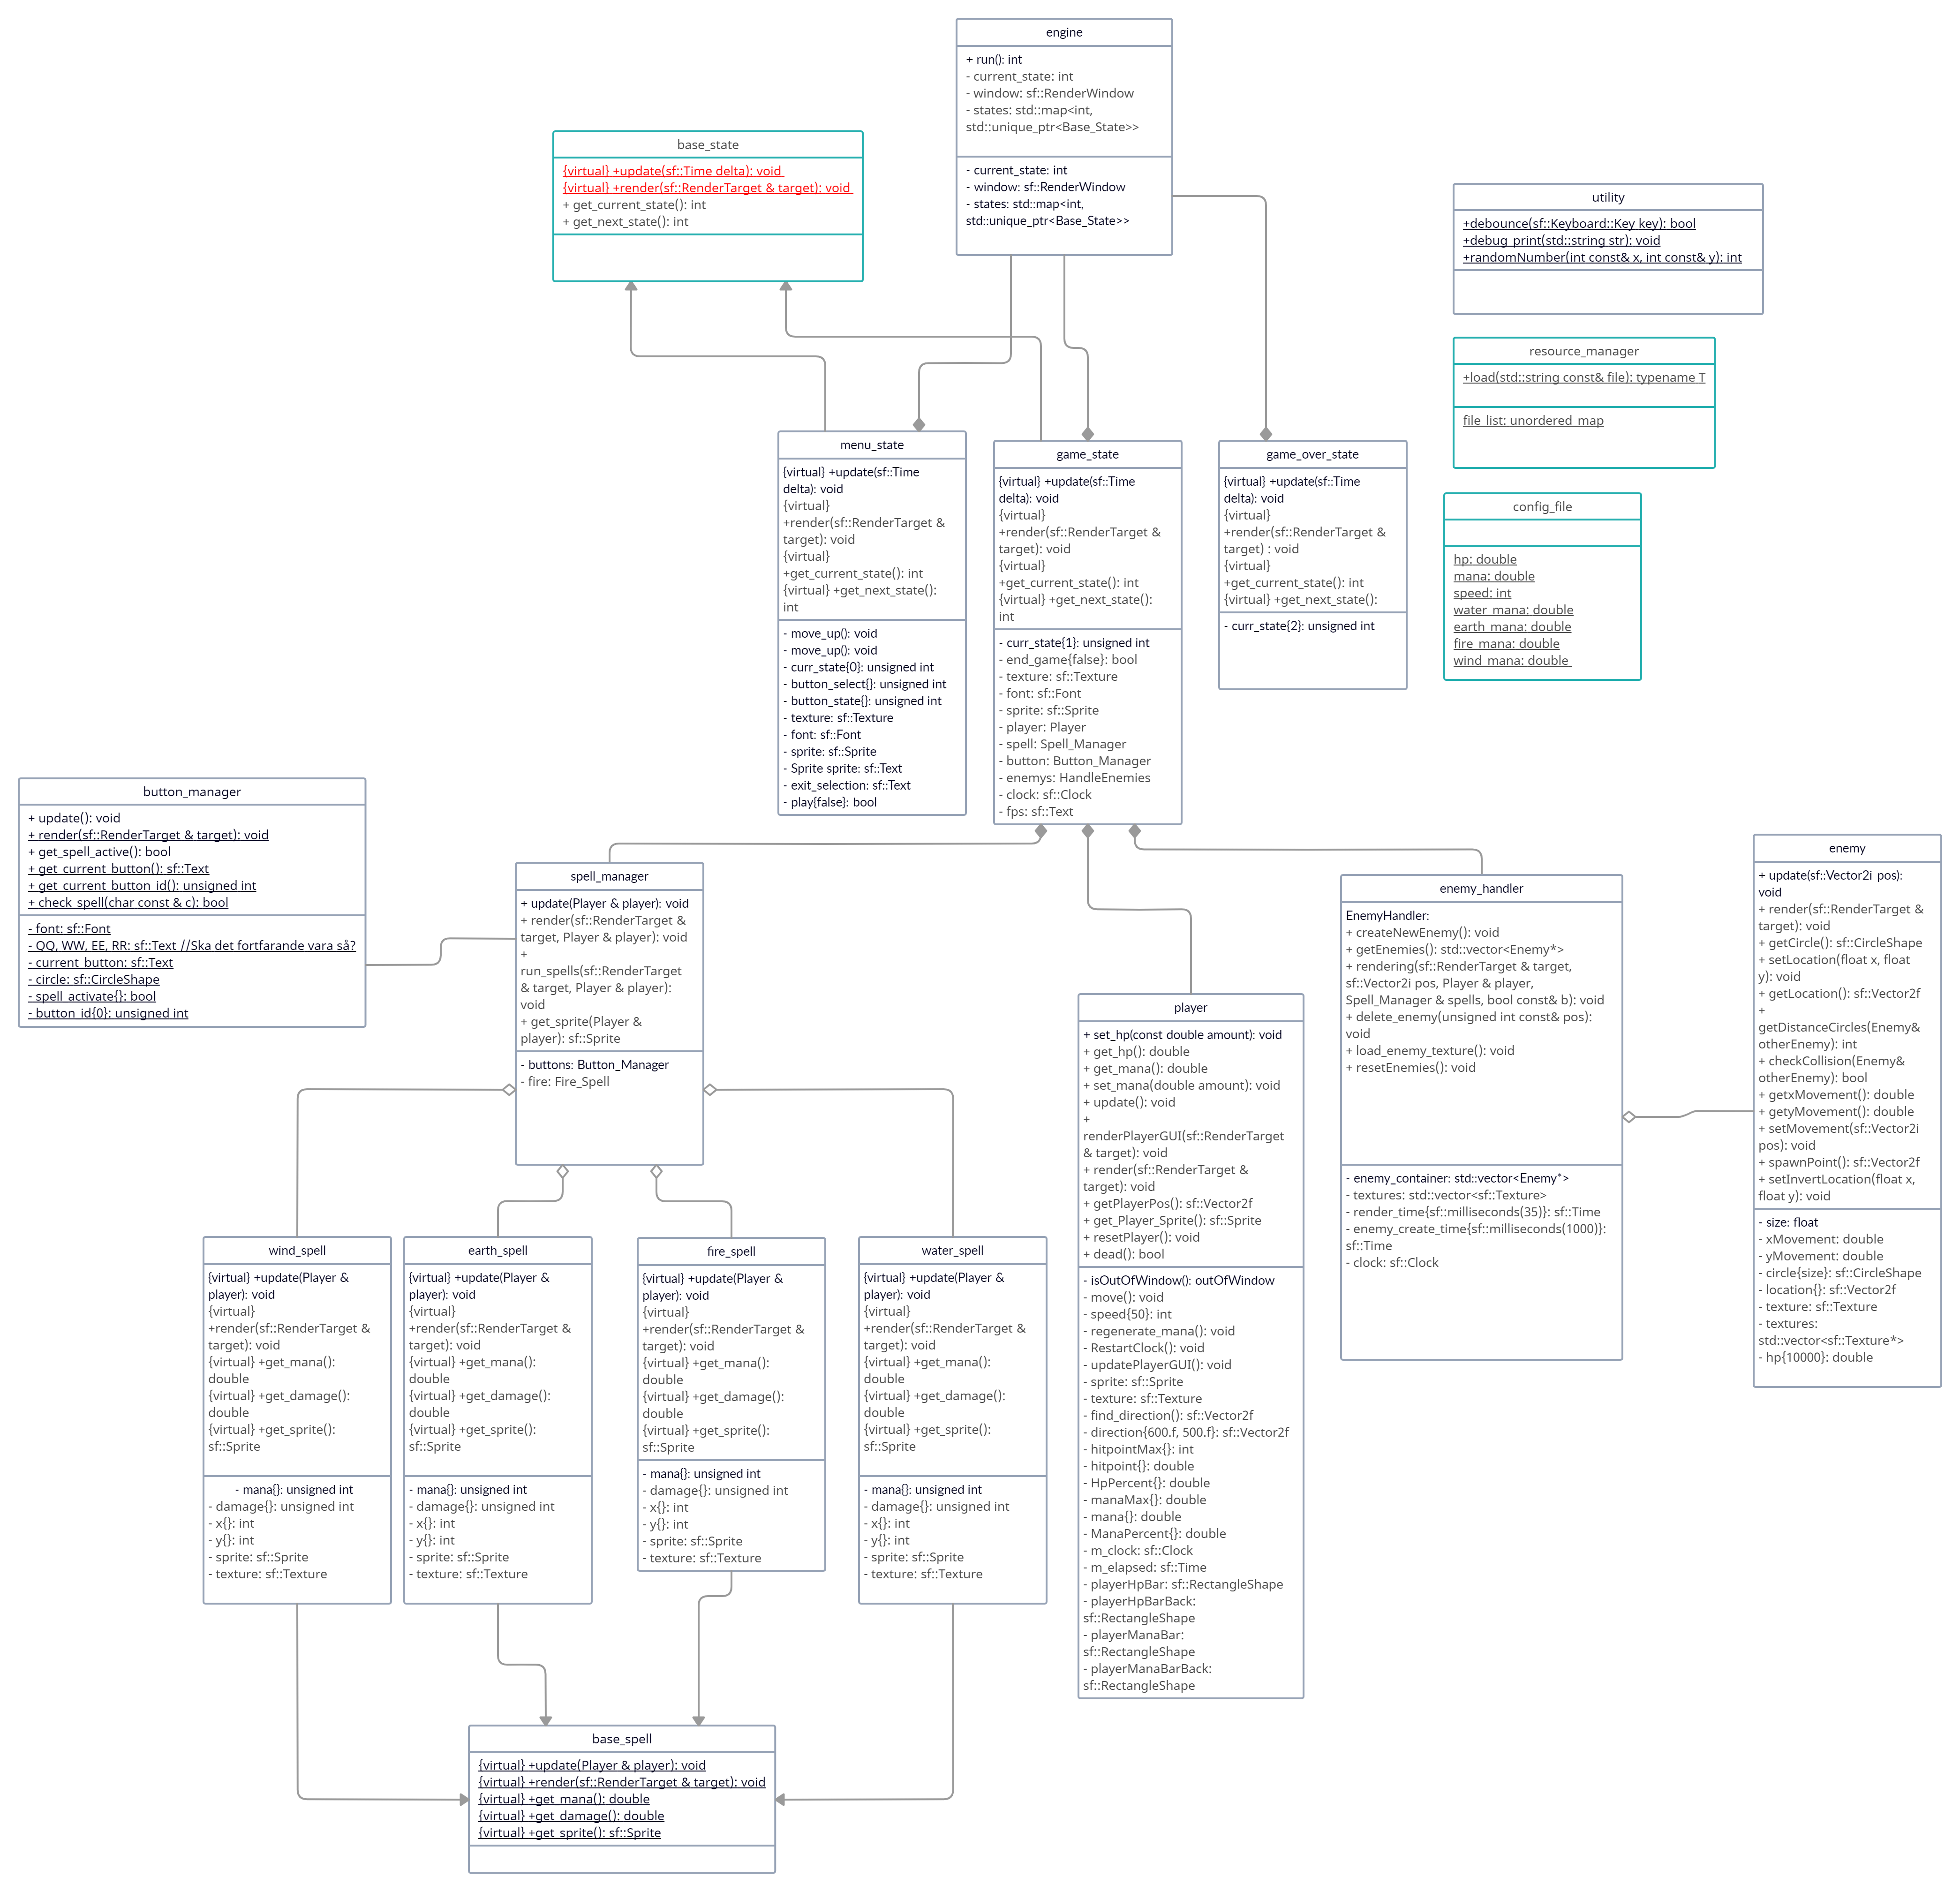
\includegraphics[scale=0.12]{uml_diagram.png}
\end{document}

